% analysis.tex
\chapter{Analysis}


\section{Problem Area}

The issue identified is the lack of mindfulness and increased forgetfulness. Keeping a journal acts as a way to document significant moments within an individual's life while providing a personal and private way for people to express their emotions. I find myself a perfect example of somebody that is lost in 'modern life,' leading me to forget even simple events which had occurred within my day. 

In a hectic world full of day-to-day distractions, the creation of a consumerist culture through the rise of social media has increased the likelihood for individuals to feel less content with their day-to-day lives. We are consuming content through different forms of media, whether that be through our computers, phones or televisions. As a result, individuals are left constantly craving to ingrain more information, but none of this information is retained. The society of the modern world has evolved to the extent that it has made it inevitable for individuals to be exposed to the high-volume of content. Such content is easily accessible through our phones,  inevitably leading individuals to become overwhelmed and overloaded. If we consider the Covid-19 quarantine and its long-lasting impact on teenagers' mental health, \cite{Imran_Aamer_Sharif_Bodla_Naveed_2020} it has left a void for individuals needing to relieve their anxieties and reduce the overall stress incorporated into their daily lives. journaling can induce a positive impact on individuals struggling with the overwhelming nature of social media and how it has clearly merged itself with day-to-day life, bringing mindfulness as a positive method in documenting and organising a person's life. 


Keeping a Journal increases productivity and mindfulness. I have always wanted to incorporate this habit into my daily routine, and through my NEA, I hope to create an easily accessible platform for myself and those alike. For my NEA, I want to create a minimal, easily navigated web-interface where individuals can add entries, storing the data, and through my web-interface, these entries can be safely stored for personal use for whoever is accessing the website. 

\subsection{Benefits of journaling}
Here are some benefits of journaling include:
\begin{itemize}
  \item It is a method of mindful writing that can help you to become more aware of your thoughts and feelings. Therefore come to terms with them.
  \item Simply jot down your thoughts and ideas, and you can come back to them later.
  \item It can help you to become more organised and productive by making you more aware of your goals and aspirations.
\end{itemize}

\bigskip

\section{Client / End User}

\newcommand{\question}[1]{\item[Q\refstepcounter{question}\thequestion.] \textit{#1}}
\newcommand{\answer}[1]{\item[A\thequestion.] #1}

journaling is an excellent habit anyone could incorporate into their daily lives. However, my primary target end-user for my app would be people like myself who are more digitally orientated and are comfortable with accessing an online platform to manage their daily lives. Teenagers and young adults are more likely to be my target audience, as they are more likely to be comfortable with using online platforms.

I've wanted to journal for quite some time now, but due to my busy schedule and overall forgetfulness, I have never been consistent with the habit for over a week. To finally properly start journaling once and for all, I will build a website front end that can be accessed as long I have an internet-connected device. This way, I can journal no matter where I am, reducing the friction that prevents me from cultivating the habit of journaling.

\subsection{Survey Result}
I have created a survey for friends and family to fill out to understand the needs and people's thoughts about journaling. Through this, I learned about more benefits of the habit and I also gained insight into people's online usage which will help me to design the app. Here are some of the results from the survey:


\begin{figure}[H]
    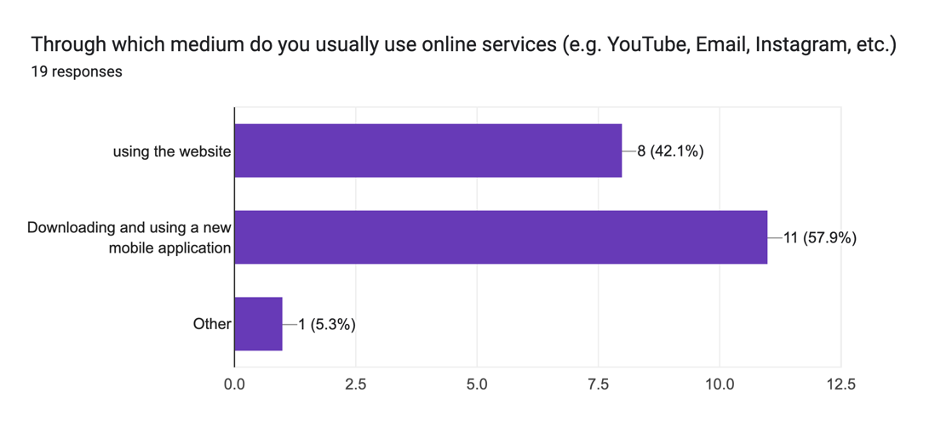
\includegraphics[width=\textwidth]{Assets/survey_medium_of_service.png}
    \caption{Survey Results Showing the Platform People Use to Access Online Services}
    \label{fig:survey_medium_of_service}
\end{figure}

The figure above shows that although most people use mobile applications to access online services, a significant number of people use website. I will be creating a website for the journal app because it's universally accessible, but in the future, I can create a mobile app to cater to the needs of the users.


\begin{figure}[H]
  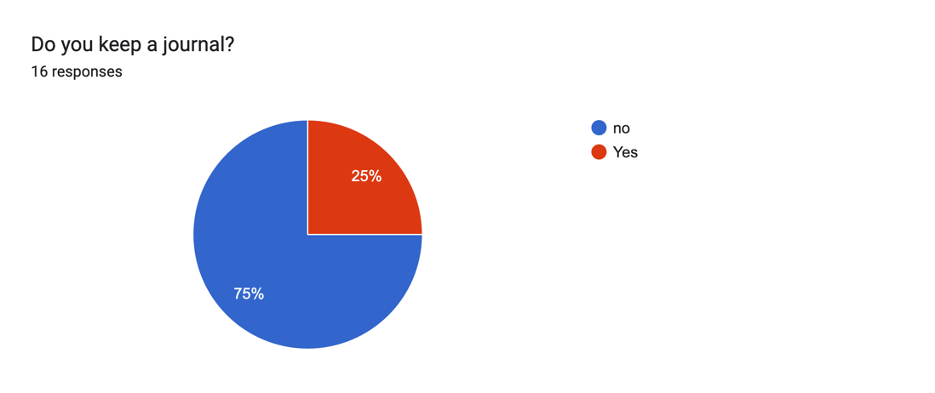
\includegraphics[width=\textwidth]{Assets/survey_keep_journal_ratio.png}
  \caption{Survey Results Showing the Ratio of People who Keep a Journal}
  \label{fig:survey_keep_journal_ratio}
\end{figure}

As expected, the majority of people do not keep a journal. Creating my app could potentially help people to start journaling and experience the benefits of the habit.


\begin{figure}[H]
    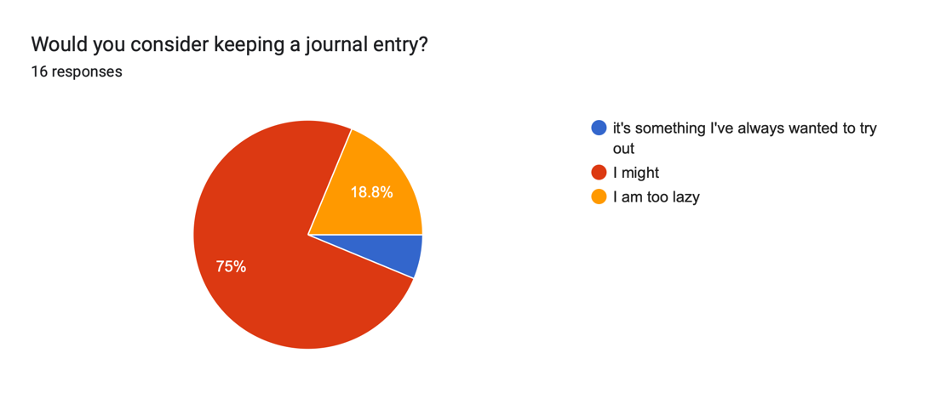
\includegraphics[width=\textwidth]{Assets/survey_consider_journal.png}
    \caption{Survey Results Showing the Ratio of People who Would Consider Journaling}
    \label{fig:survey_consider_journal}
\end{figure}

Interestingly, a significant number of people would consider journaling. This shows that there is a demand which I could potentially fill with my app.

\newcounter{question}

\newpage
\setcounter{question}{0}
\begin{itemize}
  \question{I asked the participants who journal what inspired them to start journaling.}
  \answer{}
  "I overthink too much"

  "Was more of a note taking thing I used to do then it evolved into writing - not all the time, but on occasion"

  "Having a busy period in my life where so much was going on that I realised that I wanted to remember as much of it as possible. However, I wasn't certain that I'd be able to recall everything on my own, so I wrote things down as they happened to ensure that I wouldn't forget them."

  "I was walking across the river Thames one day and I sat down for 30 minutes and just stared as the river flowed extremely peacefully. I found so many thoughts racing through my head and got restless without any digital media to entertain me. This experience inspired me to have that peace of mind and articulate my thoughts."


  \item This confirms my belief that journaling is a good habit with many benefits. 

  \question{I then asked everyone for the benefits they see in journaling.}
  \answer{Results}
  \begin{figure}[H]
    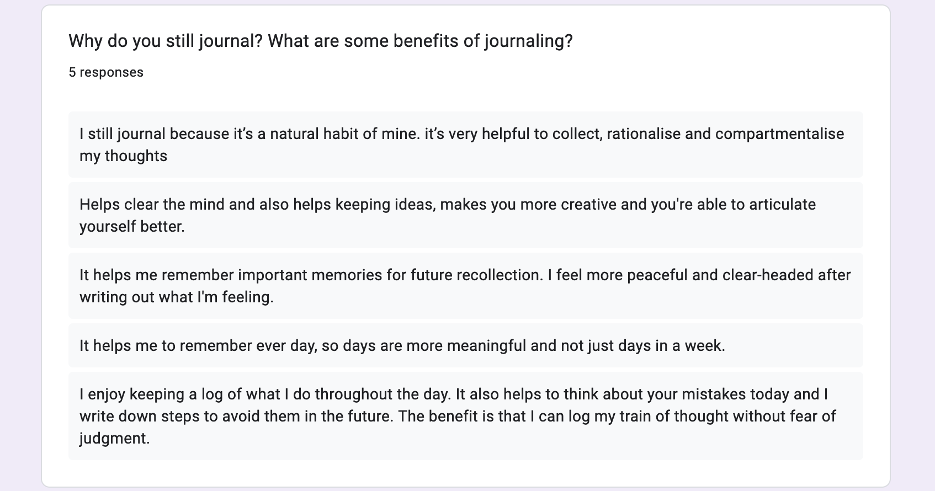
\includegraphics[width=\textwidth]{Assets/survey_benefits_journals.png}
    \caption{Survey Results Showing the Benefits of Journaling Highlighted by People Who Journal}
  \end{figure}

  \begin{figure}[H]
    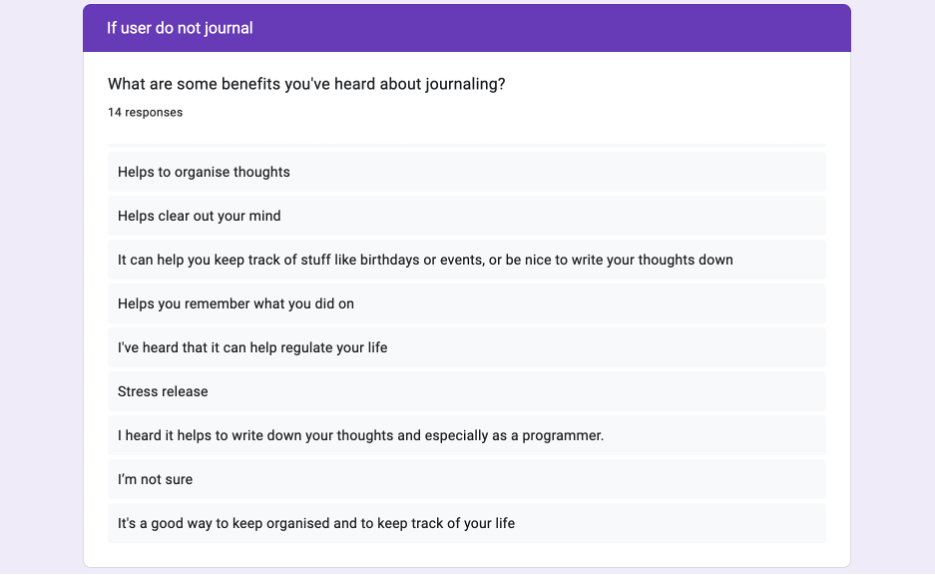
\includegraphics[width=\textwidth]{Assets/survey_benefits_not_journal.png}
    \caption{Survey Results Showing the Benefits of Journaling Highlighted by People Who Do Not Journal}
  \end{figure}

  Regardless of whether people journal or not, they all see the benefits of journaling. Almost every single person has a unanimous agreement that journaling is a good habit to have. This is a good sign for my app as I was correct for thinking that people would be interested in journaling.

  \question{Finally, I asked the participants "What would be some important and fundamental features of a digital journal app?"}
  Here are a few selected responses that represent all the responses as a whole:
  \answer{"Security, I don’t want my data to get breached and leaked."}
  \item This is a very important feature to have in the app. I will need to ensure that the data is stored securely and that sensitive information is encrypted.
  \answer{"Writing entries, being able to select and view a past date, low-key it would be really interesting to see my journaling pattern in the long term, if you can do that itd be kinda cold"}
  \item The thing to highlight here is that the user wants to be able to refer back to past entries and be able to see the statistics of their journaling. This is a good idea and I will need to implement this feature in the app.
  

\end{itemize}

\subsection*{Interview with Miss Milanova}
 I had an interview with a teacher at my school who represents someone who's slightly older than me and represents the wider user base of the app. I have picked out some responses which are particularly relevant to the application.

\setcounter{question}{0}
    \begin{itemize}
            \question{How do you feel about the security of your personal information in digital platforms? Are there expectations you have?}
            \answer{"...Yeah, surely my password and logins should be protected and private"}

            \item Users of the platform want to have a way of securely storing their sensitive information. Therefore, I will need to implement a secure way of not only storing users but also encrypting the data that is stored there. For demonstrating purposes I will be encrypting the most sensitive data such as the user's password.
            

            \question{Can you describe what you look for in a good app interface? Are there any design elements or navigation styles you find particularly helpful or annoying?}
            \answer{"...I would like to have an easy-to-use menu with options instead of a gimmicky and too-visual website."}
            \item The user wants a simple and easy-to-use interface. Therefore, I will need to design a clean and feature-rich interface. I think a navigation bar would be a good idea to implement as it clearly shows all the options available to the user.

            \question{How important is an app's speed and responsiveness to your overall user experience? Have you stopped using an app because it was too slow or unresponsive?}
            \answer{"Yes, very much it’s a waste of my time, I would rather use something else."}
            \item Performance is a key factor in the user experience. Therefore, I will need to ensure that the app is responsive and fast. I will need to use a framework that is known for its speed and performance.

            \question{How has your experience been with digital note-taking or journaling tools compared to traditional methods?}
            \answer{"No one carries a pen and paper anymore, dont be silly... Yeah [digital journaling] would be very useful for people on the go."}
            \item Website is accessible through all devices with an internet connection. Creating a website lays the foundation of the app, providing a good way for the user to do the journaling. In the future, I can add different forms of application.

            \question{Any additional comments?}
            \answer{"I find it frustrating with other apps to enter the date every time I want to log something. Can’t it just record it automatically
            Automatically - you can have your morning meeting then later you can have your evening meeting it automatically enters the date. It would be quite handy."}

            \answer{"I like it the data sync between different devices."}
            \item User wants to be able to have consistent data for ease of access. Building an API and Backend means I can store the data in a way that is easily accessible and consistent. These data can then be accessed through all forms of Frontend interfaces. This proves that in the future I can create other interfaces such as a mobile app and be able to have consistent data via the Backend.

    \end{itemize}




\section{Research Methodology}
Initially what inspired me to create a mindful journal app was when I watched a YouTube video that introduced the concept of journaling, it highlighted the vast array of benefits that journaling can bring to an individual. Then, I looked through various online articles to understand the concept a bit more. 

A reason for the creation of the app was that I wanted to create a habit of journaling, and I thought that creating an app would be a good way to do so. I have also conducted a survey and an interview to understand the needs of the user and to understand the requirements of the app.

Some of the research methods I have used include:
\begin{itemize}
  \item Surveys
  \item Interviews
  \item Watching YouTube videos
  \item Online Research
  \item Personal Experience
\end{itemize}

\section{Features of Proposed Solution}
Below I have synthesised the core features of the proposed solution. I have broken down the features into two categories - Frontend and Backend.
\section{Requirements Specification}
\begin{table}[H]
\centering
\begin{tabular}{|l|p{8cm}|p{4cm}|}
\hline
\textbf{ID} & \textbf{Requirement Description} & \textbf{How to Evidence}\\ \hline
1.1 & Develop a login page to authenticate users, include forms for user input and dynamically provide error/feedback when necessary. & Video of interaction with the app or screenshots\\ \hline

1.2 & Implement a registration page enabling new users to create an account, take in input for email, password, last name, and first name, and interact/update Backend. Provide feedback to the user after submission. & Demonstrate through UI screenshots or video, and code snippets.\\ \hline

1.3 & Develop a place where the user can see details about themselves ie their personal information and journal statistics & Provide screenshots and code snippet\\ \hline

2.1 & Create a page for users to compose new journal entries. Input parameters are the title and content of the entry. Interact with the corresponding endpoint and provide feedback to the user.& Video, screenshots, code snippets\\ \hline

2.2 & Design a retrieve journal page that lists all the user's entries, with options for sorting the entries in ascending or descending order based on creation date or other criteria in an efficient way. & Video documenting interactions with the UI, demonstrating the requried features.\\ \hline

3.1 & Implement a navigation bar that adjusts its visibility of options based on the user's login status. & Video of the UI and code snippets.\\ \hline

4.1 & Utilize state management techniques to keep the user logged in across different pages, preserving session information securely. & Screenshot and explanation of the implementation as well as video of functioning app.\\ \hline

4.2 & Handle fetching, posting, and updating data through JSON responses from the Backend. & Screenshot of code snippets showcasing a couple of examples of this in action. \\ \hline
\end{tabular}
\caption{Frontend Requirements for Journal App}
\end{table}


\begin{table}[H]
\centering
\begin{tabular}{|l|p{8cm}|p{4cm}|}  
\hline
\textbf{ID} & \textbf{Requirement Description}& \textbf{How to Evidence} \\ \hline
1.1 & Design data models for users, and journal entries, with relationships defined. & Screenshot of my database admin panel with created models and their relationship as well as code snippet of the definition of the models. \\ \hline

1.2 & Have an effective way to check the submitted user information, journal entries, and related data before storing it in the database, ensuring the data stored are in the required format. & Code snippet and testing of the functionalities. \\ \hline

1.3 & Have a way to generate statistics of the user's journaling habits, such as the most active month of the user, average entries made per week, etc. & Code snippet of the function that generates the statistics and screenshots of the statistics being displayed. \\ \hline

2.1 & Develop API endpoints with functionalities implemented to handle user authentication (login and registration) and other core endpoints that drive the journal app as a whole & use tools to run requests against the endpoints and capture their responses, testing different cases.\\ \hline

2.2 & Features for secure password storage(salting and hashing) and and authenticate; token generation for session management.& Run tests to see the functionalities are working\\ \hline

3.1 & Ensure all API endpoints are secured and accessible only to authenticated users, using tokens or similar mechanisms for session management.& screenshots of authenticated requests and their responses. \\ \hline

3.2 & Ensure smooth and spontaneous communication with the Frontend. & Provide video of the working application \\ \hline

4.1 & Design the Backend with room for more functionalities & Code snippets of non-core functionalities being implemented. \\ \hline

\end{tabular}
\caption{Backend Requirements for Journal App}
\end{table}

\pagebreak

\section{Critical Path}
The critical path refers to the sequence of the stages in the development of my application. I am doing full stack development, which includes independent Backend and Frontend both with many small features to add all the time. The Agile methodology would be suitable for me to follow for my project. This is because it is a flexible and iterative approach that allows repeated tests of all the small modules and eventually builds up to a complete solution. It is also a good way to manage the project as I can easily adapt to changes, and I will need to make many changes since there will be many new things I will learn and obstacles overcome to as I am developing the app.

\bigskip

\begin{figure}[H]
    \centering
    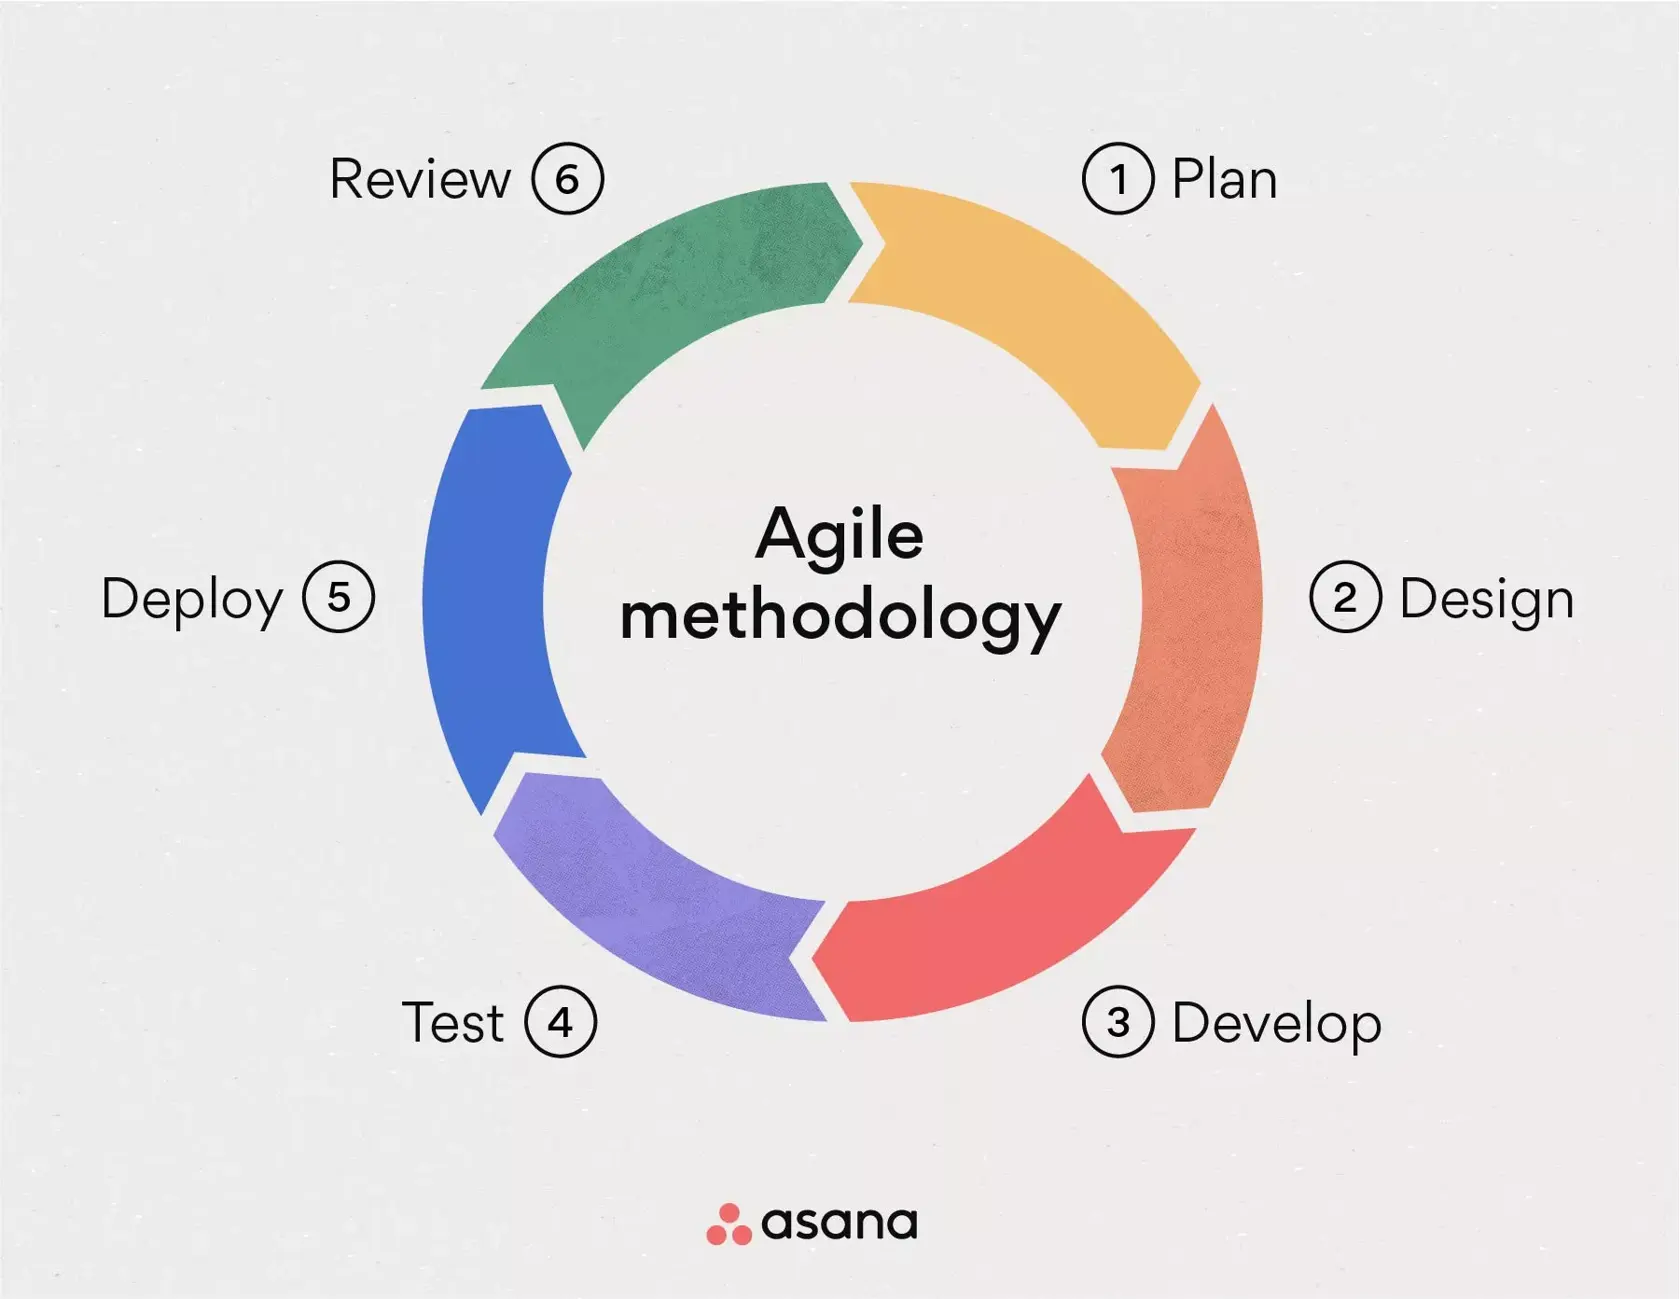
\includegraphics[width=0.8\textwidth]{Assets/Agile_asana.png}
    \caption{Imagine Showing the Steps of the Agile Methodology taken from \cite{laoyan2024agile}}
    \label{fig:critical_path}
\end{figure}